\vspace{-0.6\baselineskip}
\section{Task and motivation}
\vspace{-0.4\baselineskip}
\label{sec:intro}

With the advances of deep learning techniques and data collection, there have been successes in scaling up object classification systems. However, unlike object classification, diverse object classes and tedious bounding boxes annotation are hardly scalable. Recently, there have been impressive progresses in unsupervised and weakly supervised object detection, getting rid of the tediou bounding box annotation process. However, existing unsupervised methods show much inferior performance compared to supervised methods. And the weakly supervised ones fail to generalize to videos due to domain shift. In this paper, we focus on the problem of ``weakly supervised object detection by learning from action labes''. Only videos with action labels are used for training and the test output includes bounding boxes on static images/frames.

We are motivated by the observation that object appearance is consistent across videos of same action class and also across action classes which involve the same object class. \figref{fig:motivation1} shows the same object ``cup/bottle'' appearing in 4 different actions. The motion of subject and object is also consistent within the same action class. For example in the action ``tidy up with a broom'', the motion of object broom often includes swinging around while the motion of subject involves the arm moving foreward and backward. 

\begin{figure}
% \vspace{-0.5\baselineskip}
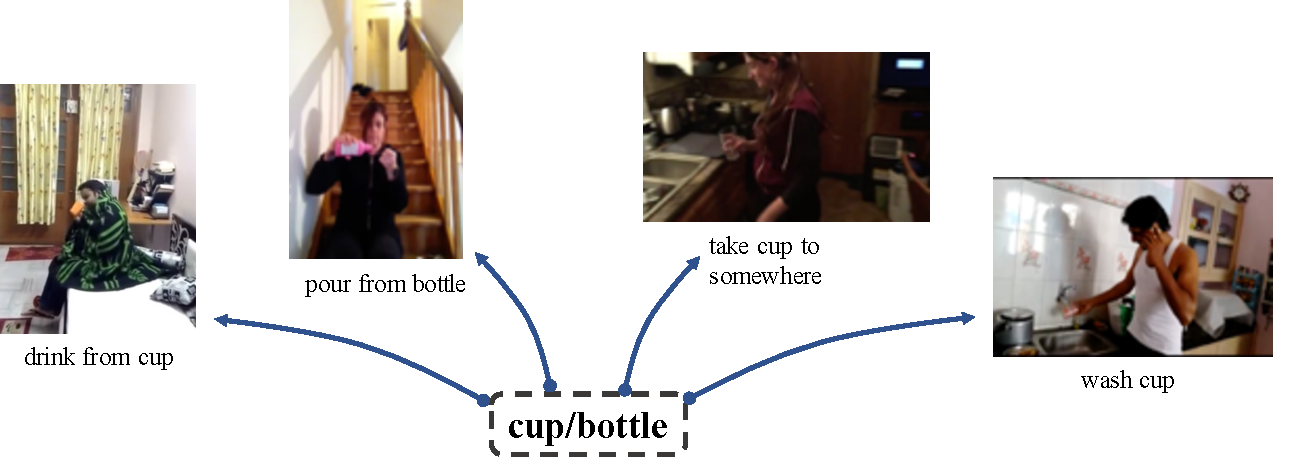
\includegraphics[width=0.48\textwidth]{figures/sameobj_differentaction.pdf}
% \caption{Visual comparison of depth and normal results between \protect\cite{zhou2017unsupervised} and ours. As the original depth ground truth map comes from sparse laser measurement, the interpolated depth map is shown for better visualization. As can be seen from the depth estimation, our results preserve the small/thin structures which have similar color to other foregrounds (green circles). From the normal comparison, our results predict the road normal direction better and have no artifact. The edges in normal map are also preserved better in our results (yello circles).}
\caption{Different actions interact with objects of the same class.}
% \vspace{-0.8\baselineskip}
\label{fig:motivation1}
\end{figure}


